% \begin{figure*}[!t]
%     \centering
%     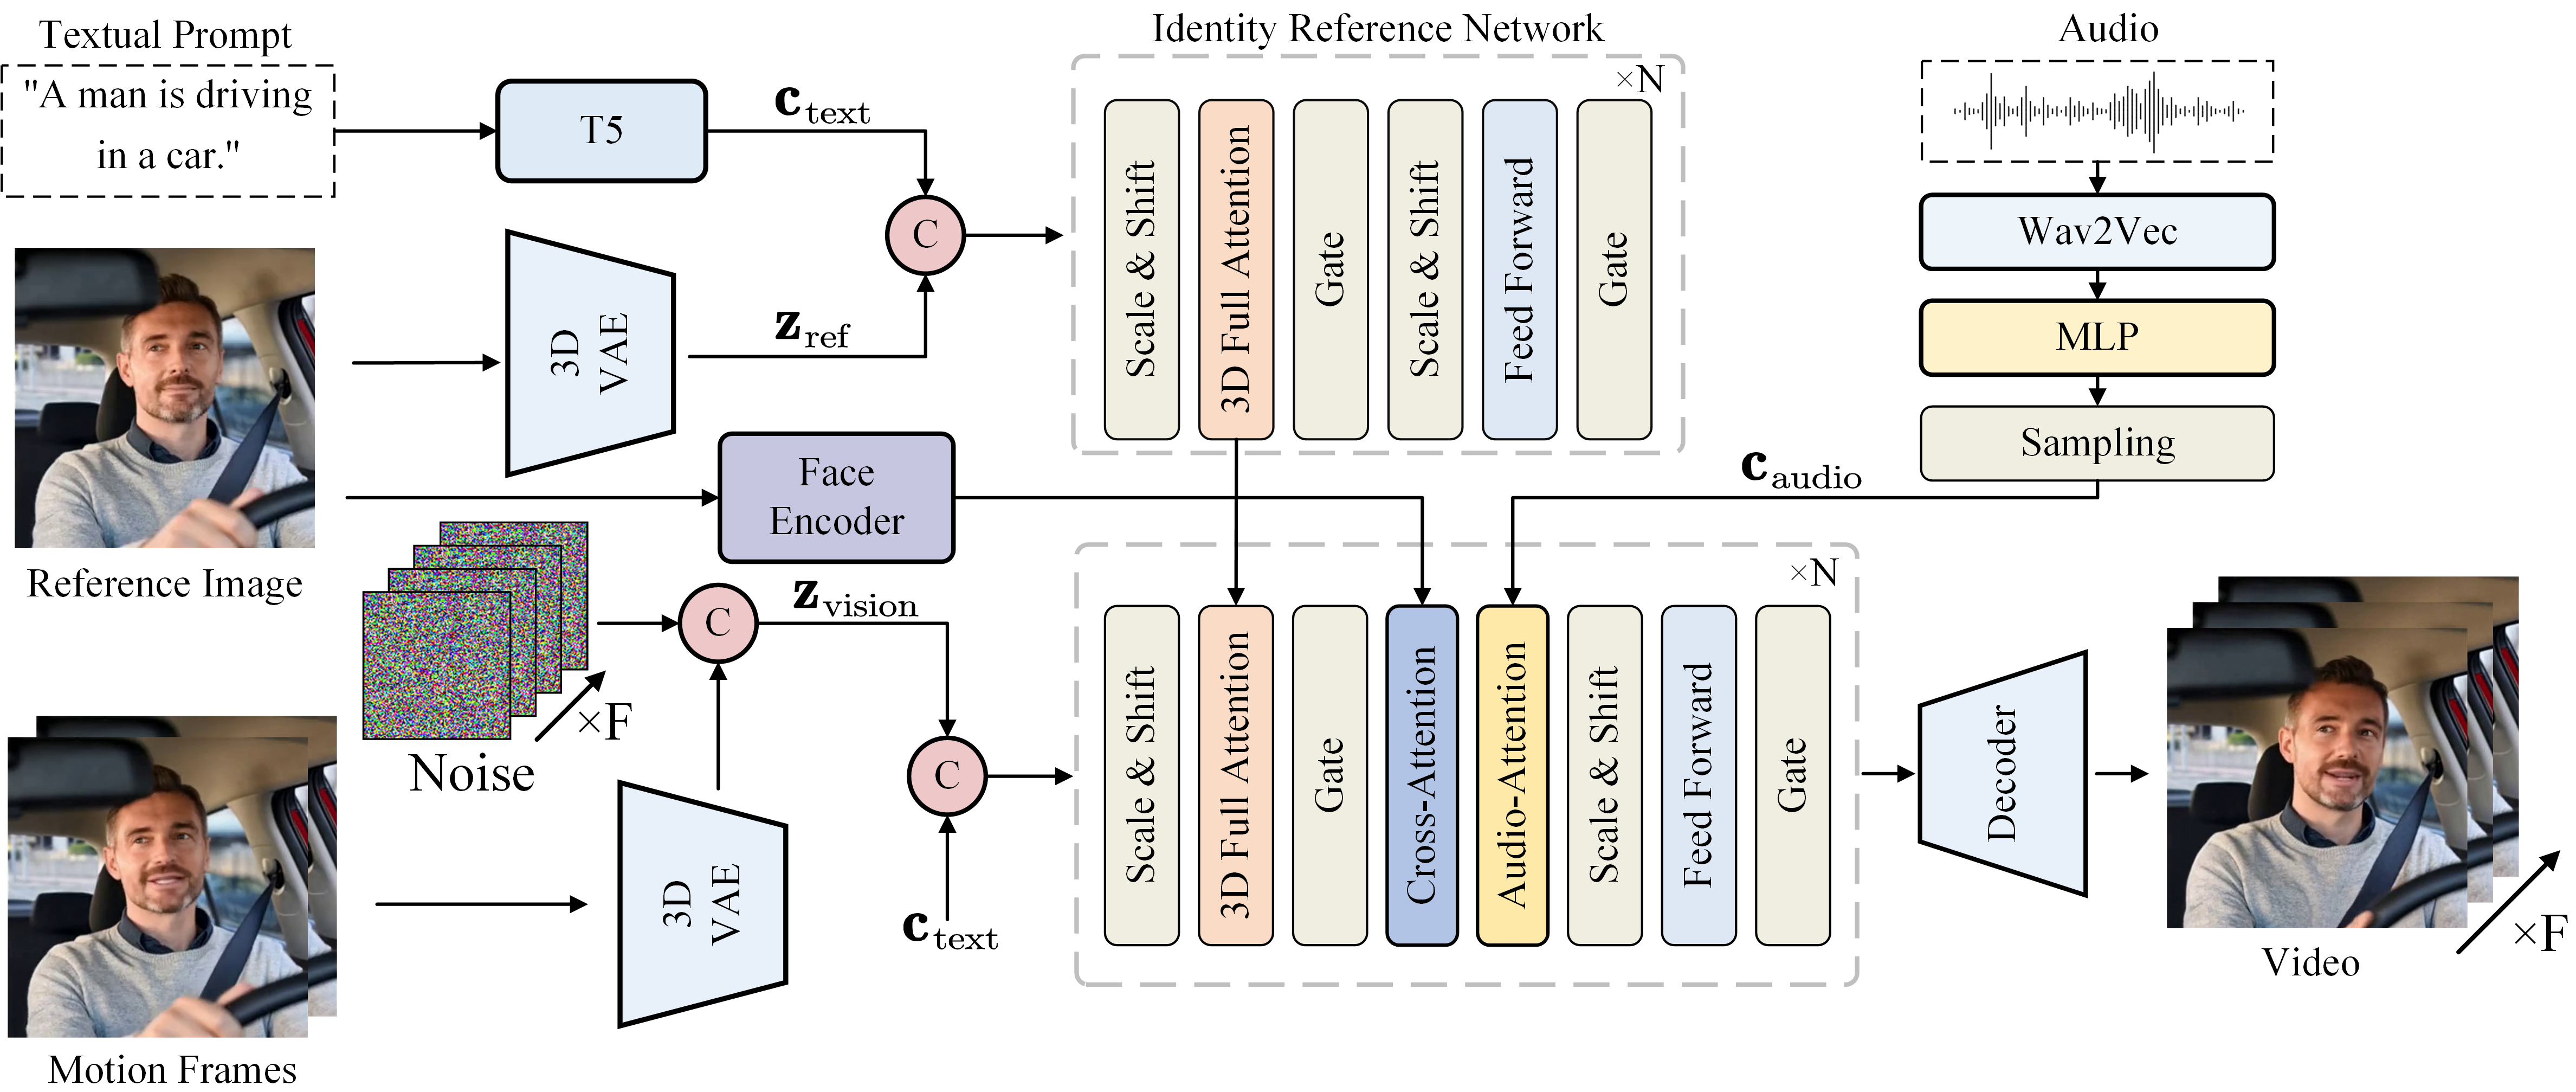
\includegraphics[width=1\linewidth]{figs/Pipeline.png}
%     \caption{The overview of the proposed method. Specifically, the method takes reference images, an audio sequence, and textual prompts as inputs to generate a video output with temporal consistency and high visual fidelity. We leverage the casual 3D VAE, T5, and Wav2Vec models to process the visual, textual, and audio features, respectively. The Identity Reference Network extracts identity features from the input reference images and textual prompts, enabling controllable animation while preserving the subject's appearance. The audio encoder generates motion information for lip synchronization, while the face encoder extracts facial features to maintain consistency in facial expressions. The 3D Full Attention and Audio-Attention Modules combine identity and motion data within a denoising network, producing high-fidelity, temporally consistent, and controllable animated videos.}
%     \label{fig:architecture}
%     \vspace{-4 mm}
% \end{figure*}


\begin{figure*}[t!]
    \centering

    % 左侧大图
    \begin{minipage}[b]{0.65\textwidth} % 左侧宽度占40%
        \centering
        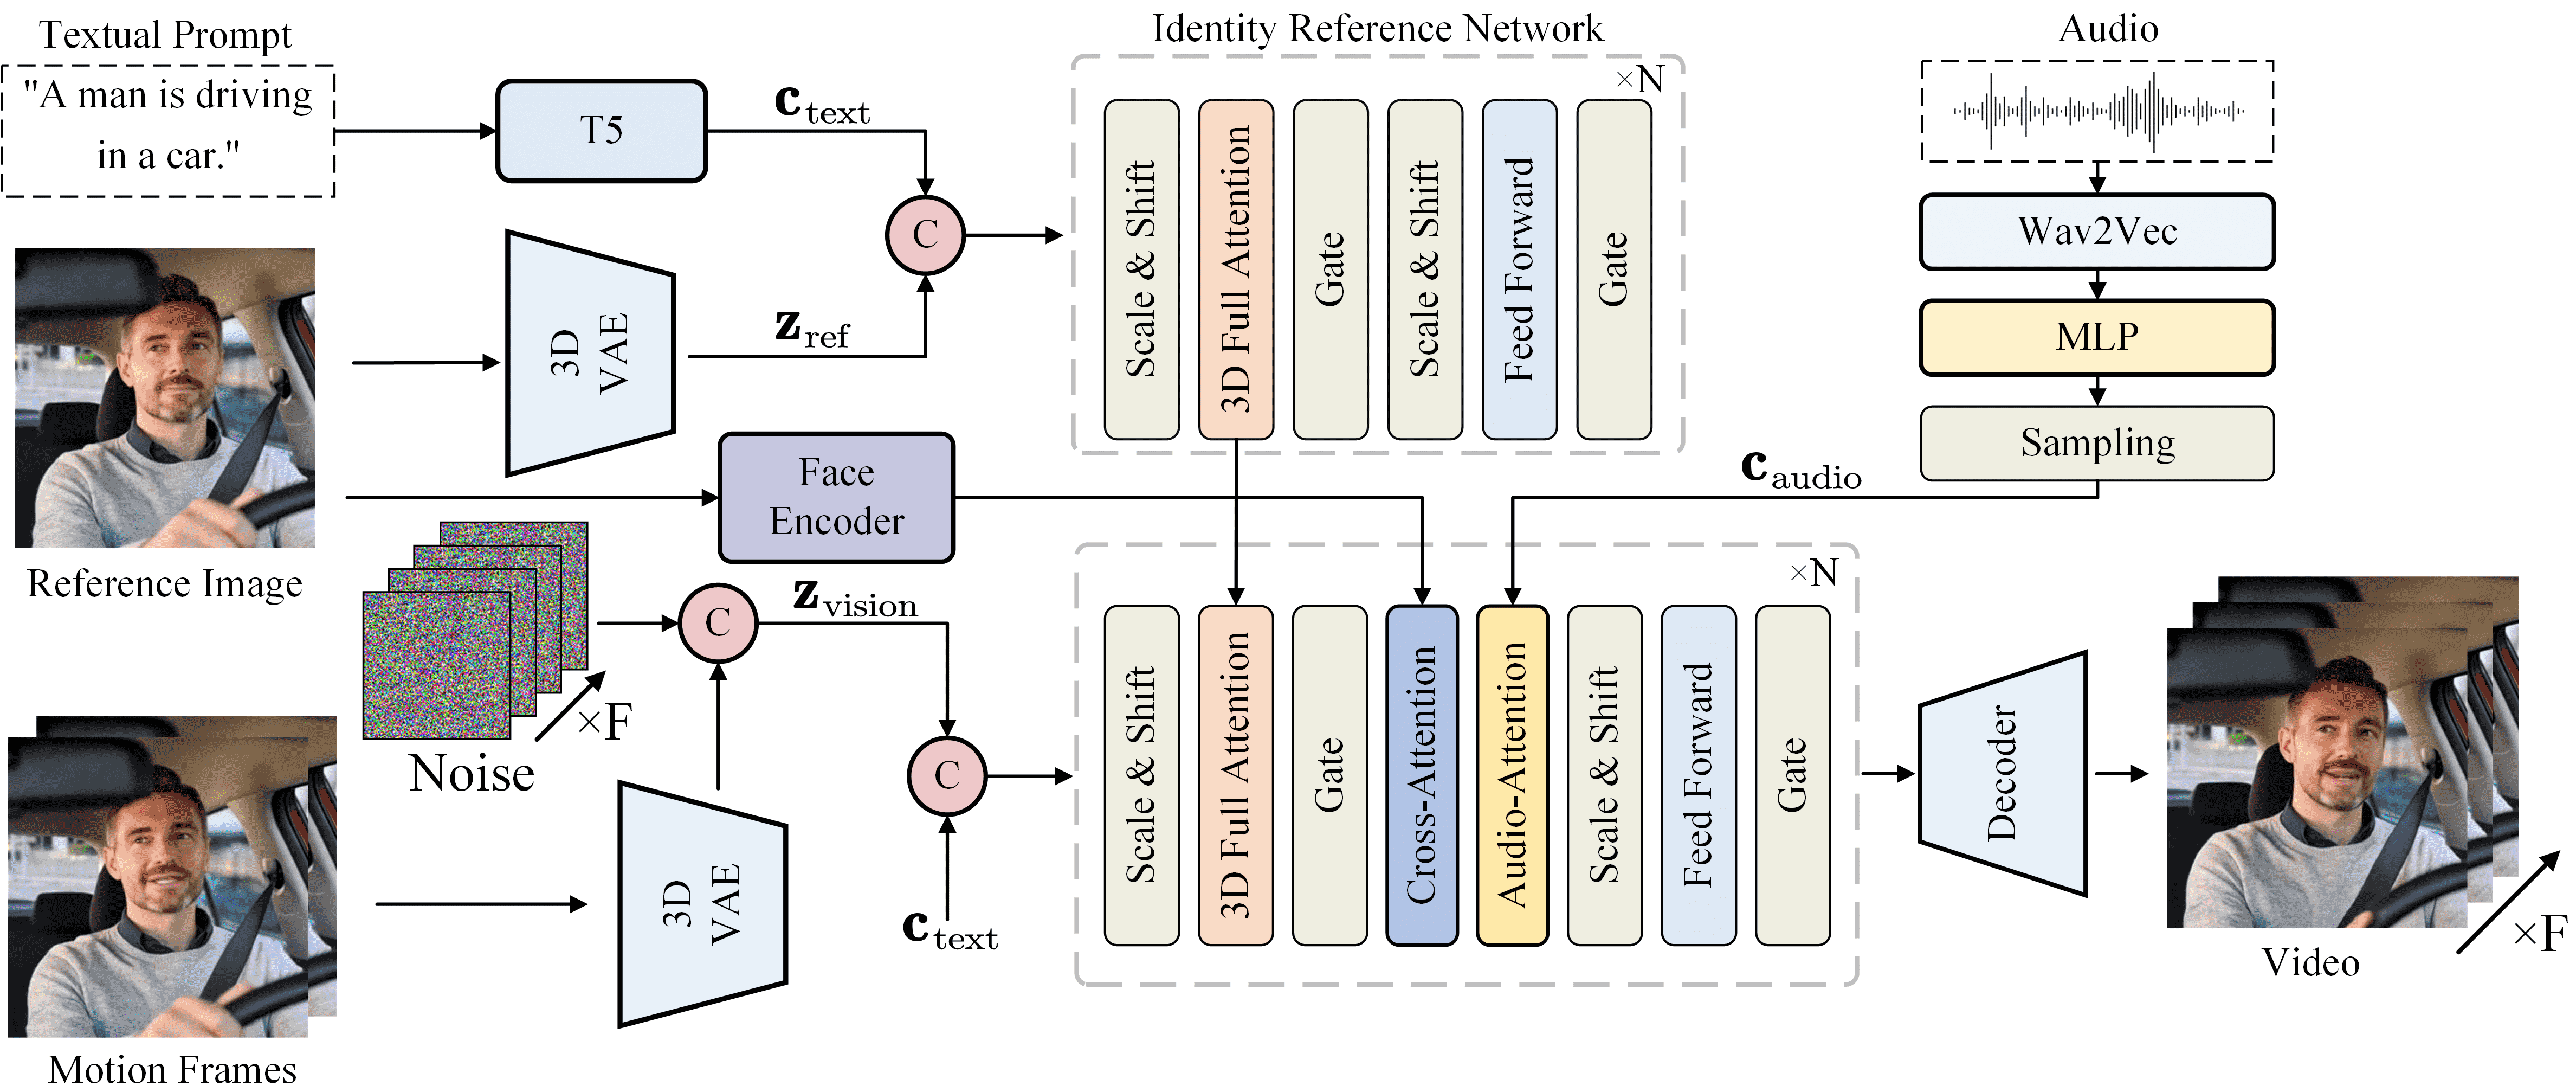
\includegraphics[width=\linewidth]{figs/Pipeline_comp.png} % 替换为你的图片路径
        \caption{The overview of the proposed method. Specifically, the method takes a reference image, an audio sequence, and a textual prompt as inputs to generate a video output with temporal consistency and high visual fidelity. We leverage the casual 3D VAE, T5, and Wav2Vec models to process the visual, textual, and audio features, respectively. The Identity Reference Network extracts identity features from the input reference image and textual prompt, enabling controllable animation while preserving the subject's appearance. The audio encoder generates motion information for lip synchronization, while the face encoder extracts facial features to maintain consistency in facial expressions. The 3D Full Attention and Audio-Attention Modules combine identity and motion data within a denoising network, producing high-fidelity, temporally consistent, and controllable animated videos.}
        \label{fig:architecture}

    \end{minipage}
    \hfill
    % 右侧上下两张小图
    \begin{minipage}[b]{0.32\textwidth} % 右侧宽度占55%
        \centering
        \begin{minipage}[b]{\textwidth} % 上方图
                \centering
                \begin{subfigure}{0.3\linewidth} % 增加 subfigure 的宽度
                    \centering
                    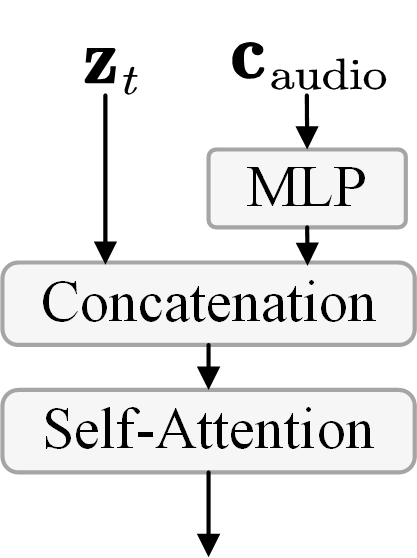
\includegraphics[width=\linewidth]{figs/AudioCondition/Audio_SA.png} 
                    \caption{}  
                    \label{fig:AudioConditionSA}  
                \end{subfigure}%
                \hfill
                \begin{subfigure}{0.3\linewidth} % 增加 subfigure 的宽度
                    \centering
                    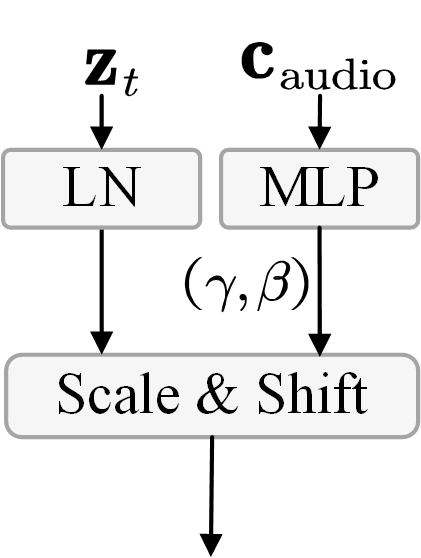
\includegraphics[width=\linewidth]{figs/AudioCondition/Audio_Ada.png}  
                    \caption{}  
                    \label{fig:AudioConditionAda}  
                \end{subfigure}%
                \hfill
                \begin{subfigure}{0.3\linewidth} % 增加 subfigure 的宽度
                    \centering
                    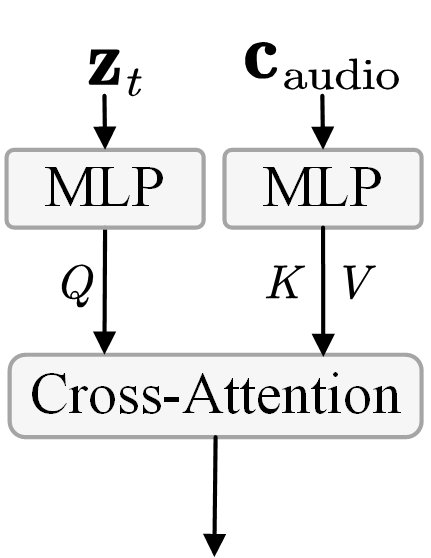
\includegraphics[width=\linewidth]{figs/AudioCondition/Audio_CA.png}  
                    \caption{}  
                    \label{fig:AudioConditionCA}  
                \end{subfigure}%
                \vspace{-1mm}
                \caption{Different strategies of audio conditioning. (a) self-attention; (b) adaptive norm; (c) cross-attention.}
                \label{fig:AudioCondition}
        \end{minipage}
        % \vspace{0.5cm} % 上下图片间距
        \begin{minipage}[b]{\textwidth} % 下方图
            \centering
            \begin{subfigure}{0.22\linewidth} % 增加 subfigure 的宽度
                \centering
                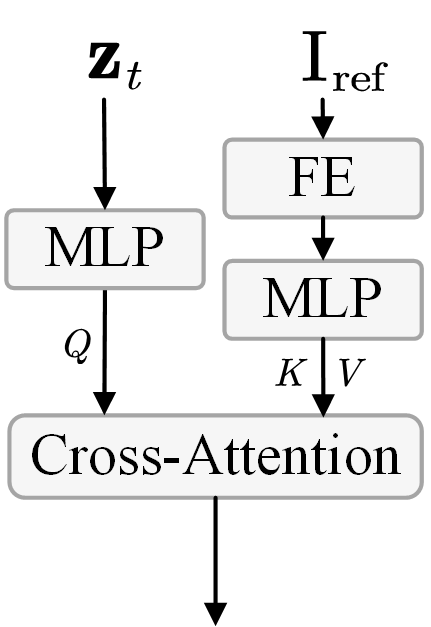
\includegraphics[width=0.95\linewidth]{figs/RefCondition/FE_CA.png} 
                \caption{}  
                \label{fig:RefConditionCA}  
            \end{subfigure}%
            \hfill
            \begin{subfigure}{0.22\linewidth} % 增加 subfigure 的宽度
                \centering
                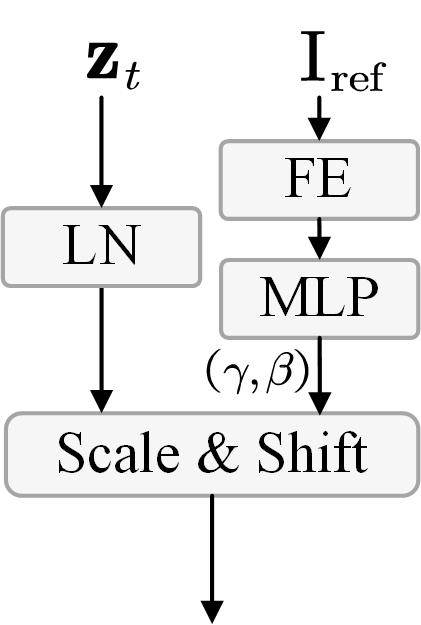
\includegraphics[width=0.95\linewidth]{figs/RefCondition/FE_Ada.png}  
                \caption{}  
                \label{fig:RefConditionAda}  
            \end{subfigure}%
            \hfill
            \begin{subfigure}{0.23\linewidth} % 增加 subfigure 的宽度
                \centering
                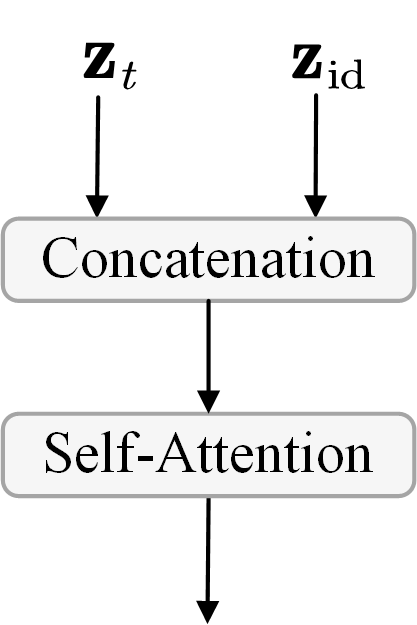
\includegraphics[width=0.95\linewidth]{figs/RefCondition/VAE_SA.png}  
                \caption{}  
                \label{fig:RefConditionVAESA}  
            \end{subfigure}%
            \hfill
            \begin{subfigure}{0.30\linewidth} % 增加 subfigure 的宽度
                \centering
                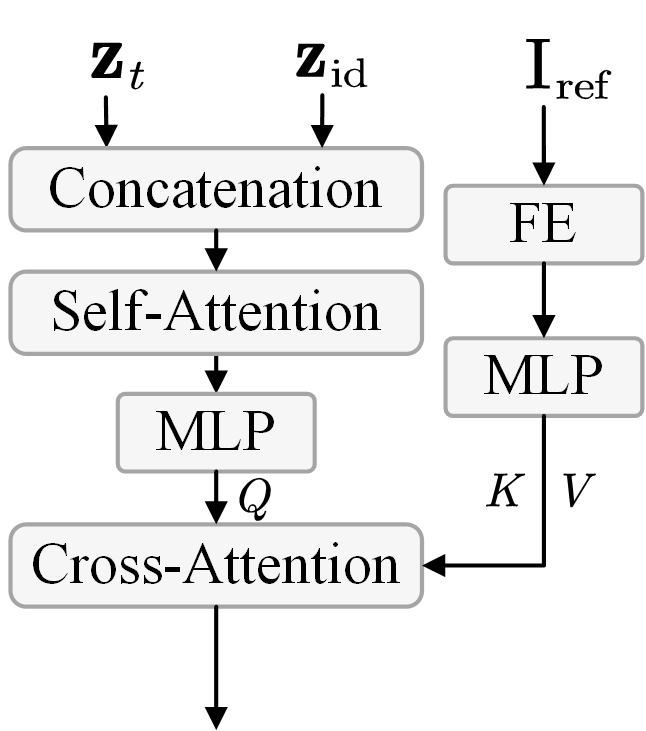
\includegraphics[width=\linewidth]{figs/RefCondition/VAE_CA.png}  
                \caption{}  
                \label{fig:RefConditionVAECA}  
            \end{subfigure}%
             \label{fig:RefCondition}
             \vspace{-1mm}
            \caption{{Different strategies of identity conditioning. FE refers to the face encoder. cross-attention demonstrates the best performance. (a) face attention; (b) face adaptive norm; (c) identity reference network; (d) face attention and identity reference network.}}
            \label{fig:IdCondition}
        \end{minipage}
    \end{minipage}
    % \vspace{5mm}
\end{figure*}


 
\section{Methodology}  
This methodology section systematically outlines the approaches employed in our study. 
Section~\ref{sec:baseline} describes the baseline transformer diffusion network, detailing its architecture and functionality. 
Section~\ref{sec:audio} focuses on the integration of speech audio conditions via a cross-attention mechanism. 
Section~\ref{sec:identity} discusses the implementation of the identity reference network, which is crucial for preserving facial identity coherence throughout extended video sequences. 
Section~\ref{sec:train} reviews the training and inference procedures used for the transformer diffusion network. 
Finally, Section~\ref{sec:data} details the comprehensive strategies for data sourcing and preprocessing.

\subsection{Baseline Transformer Diffusion Network}\label{sec:baseline}
\noindent\textbf{Baseline Network.}  
The CogVideoX model~\cite{yang2024cogvideox} serves as the foundational architecture for our transformer diffusion network, employing a 3D VAE for the compression of video data. 
In this framework, latent variables are concatenated and reshaped into a sequential format, denoted as \(\mathbf{z}_t\). 
Concurrently, the model utilizes the T5 architecture~\cite{raffel2023t5} to encode textual inputs into embeddings, represented as \(\mathbf{c}_{\text{text}}\). 
The combined sequences of video latent representations \(\mathbf{z}_t\) and textual embeddings \(\mathbf{c}_{\text{text}}\) are subsequently processed through an expert transformer network. 
To address discrepancies in feature space between text and video, we implement expert adaptive layer normalization techniques, which facilitate the effective utilization of temporal information and ensure robust alignment between visual and semantic data. 
Following this integration, a repair mechanism is applied to restore the original latent variable, after which the output is decoded through the 3D causal VAE decoder to reconstruct the video. 
Furthermore, the incorporation of 3D Rotational Positional Encoding (3D RoPE)~\cite{yang2024cogvideox} enhances the model's capacity to capture inter-frame relationships across the temporal dimension, thereby establishing long-range dependencies within the video framework.  

\noindent\textbf{Conditioning in Diffusion Transformer.}  
In addition to the textual prompt \(\mathbf{c}_{\text{text}}\), we introduce two supplementary conditions: the speech audio condition \(\mathbf{c}_{\text{audio}}\) and the identity appearance condition \(\mathbf{c}_{\text{id}}\).  

Within diffusion transformers, four primary conditioning mechanisms are identified: in-context conditioning, cross-attention, adaptive layer normalization (adaLN), and adaLN-zero~\cite{Peebles2022DiT}. 
Our investigation primarily focuses on cross-attention and adaptive layer normalization (adaLN). Cross-attention enhances the model's focus on conditional information by treating condition embeddings as keys and values, while latent representations serve as queries. 
Although adaLN is effective in simpler conditioning scenarios, it may not be optimal for more complex conditional embeddings that incorporate richer semantic details, such as sequential speech audio. Relevant comparative analyses will be elaborated upon in the experimental section.  

\subsection{Audio-Driven Transformer Diffusion}\label{sec:audio}
\noindent\textbf{Speech Audio Embedding.}  
To extract salient audio features for our proposed model, we utilize the wav2vec framework developed by Schneider et al.~\cite{schneider2019wav2vec}. The audio representation is defined as \(\mathbf{c}_{\text{audio}}\). 
Specifically, we concatenate the audio embeddings generated by the final twelve layers of the wav2vec network, resulting in a comprehensive semantic representation capable of capturing various audio hierarchies. 
This concatenation emphasizes the significance of phonetic elements, such as pronunciation and prosody, which are crucial as driving signals for character generation. 
To transform the audio embeddings obtained from the pretrained model into frame-specific representations, we apply three successive linear transformation layers, mathematically expressed as: $\mathbf{c}_{\text{audio}}^{(f)} = \mathcal{L}_3 \left( \mathcal{L}_2 \left( \mathcal{L}_1 \left( \mathbf{c}_{\text{audio}} \right) \right) \right)$, where \(\mathcal{L}_1\), \(\mathcal{L}_2\), and \(\mathcal{L}_3\) represent the respective linear transformation functions. This systematic approach ensures that the resulting frame-specific representations effectively encapsulate the nuanced audio features essential for the performance of our model.  

% \begin{figure}[th!]
% \vspace{-2mm}
%     \centering
%     \begin{subfigure}{0.3\linewidth} % 增加 subfigure 的宽度
%         \centering
%         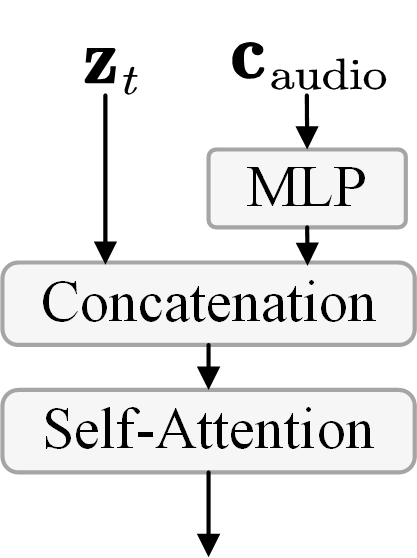
\includegraphics[width=\linewidth]{figs/AudioCondition/Audio_SA.png} 
%         \caption{Self-Attention}  
%         \label{fig:AudioConditionSA}  
%     \end{subfigure}%
%     \hfill
%     \begin{subfigure}{0.3\linewidth} % 增加 subfigure 的宽度
%         \centering
%         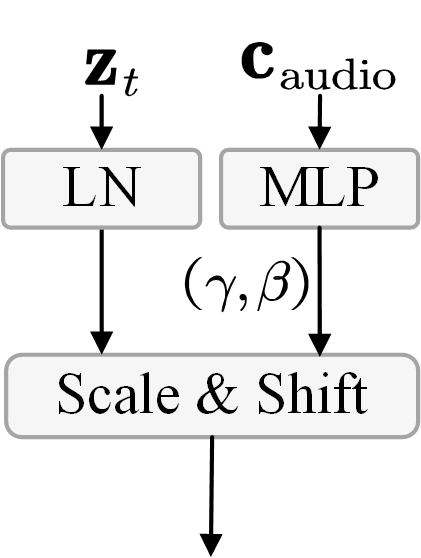
\includegraphics[width=\linewidth]{figs/AudioCondition/Audio_Ada.png}  
%         \caption{Adaptive Norm}  
%         \label{fig:AudioConditionAda}  
%     \end{subfigure}%
%     \hfill
%     \begin{subfigure}{0.3\linewidth} % 增加 subfigure 的宽度
%         \centering
%         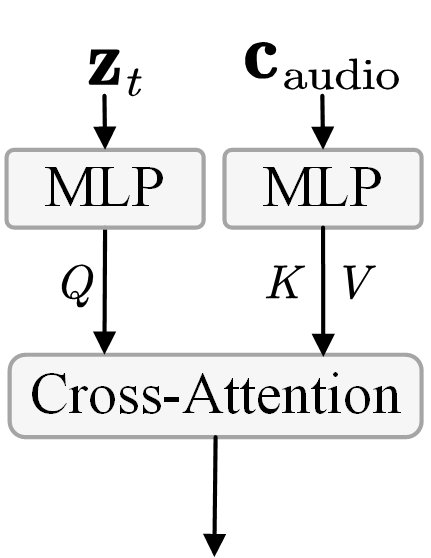
\includegraphics[width=\linewidth]{figs/AudioCondition/Audio_CA.png}  
%         \caption{Cross-Attention}  
%         \label{fig:AudioConditionCA}  
%     \end{subfigure}%
    
%     \caption{Different strategies of audio conditioning. Cross-Attention demonstrates the best performance.}
%     \label{fig:AudioCondition}
%     \vspace{-4mm}
% \end{figure}


\noindent\textbf{Speech Audio Conditioning.}  
We explore three fusion strategies---self-attention, adaptive normalization, and cross-attention---as illustrated in Figure~\ref{fig:AudioCondition} to integrate audio condition into the DiT-based video generation model. Our experiments show that the cross-attention strategy delivers the best performance in our model. For more details, please refer to Section~\ref{sec:ablationstudy}. 

Following this, 
 we integrate audio attention layers after each face-attention layer within the denoising network, employing a cross-attention mechanism that facilitates interaction between the latent encodings and the audio embeddings. 
Specifically, within the DiT block, the motion patches function as keys and values in the cross-attention computation with the hidden states \(\mathbf{z}_t\): $\mathbf{z}_t = \text{CrossAttention}(\mathbf{z}_t, \mathbf{c}_{\text{audio}}^{(f)})$. This methodology leverages the conditional information from the audio embeddings to enhance the coherence and relevance of the generated outputs, ensuring that the model effectively captures the intricacies of the audio signals that drive character generation.  




\subsection{Identity Consistent Transformer Diffusion}\label{sec:identity}

% \begin{figure}[th!]
%     \centering
%     \begin{subfigure}{0.22\linewidth} % 增加 subfigure 的宽度
%         \centering
%         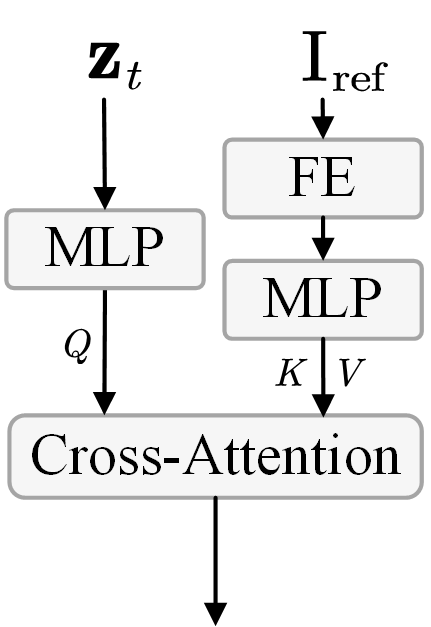
\includegraphics[width=0.95\linewidth]{figs/RefCondition/FE_CA.png} 
%         \caption{}  
%         \label{fig:RefConditionCA}  
%     \end{subfigure}%
%     \hfill
%     \begin{subfigure}{0.22\linewidth} % 增加 subfigure 的宽度
%         \centering
%         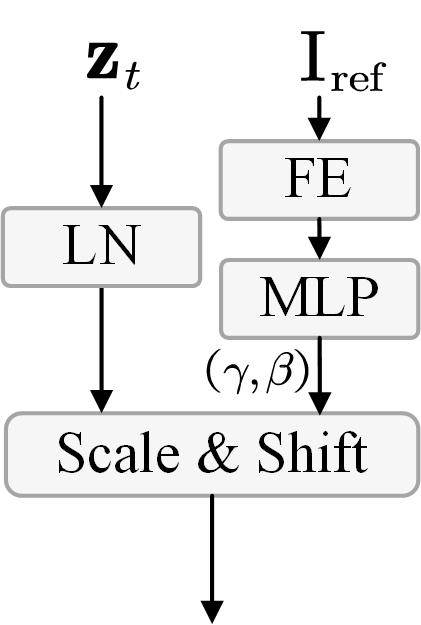
\includegraphics[width=0.95\linewidth]{figs/RefCondition/FE_Ada.png}  
%         \caption{}  
%         \label{fig:RefConditionAda}  
%     \end{subfigure}%
%     \hfill
%     \begin{subfigure}{0.23\linewidth} % 增加 subfigure 的宽度
%         \centering
%         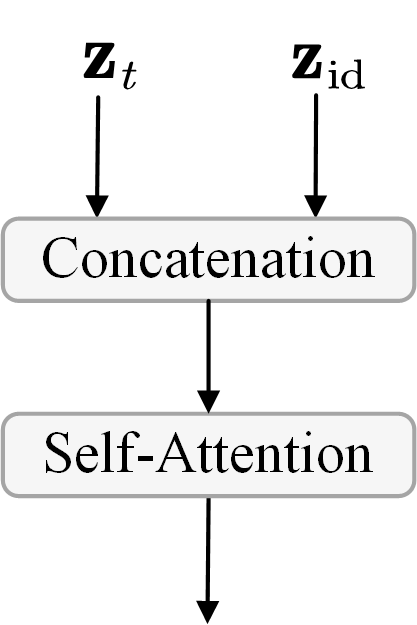
\includegraphics[width=0.95\linewidth]{figs/RefCondition/VAE_SA.png}  
%         \caption{}  
%         \label{fig:RefConditionVAESA}  
%     \end{subfigure}%
%     \hfill
%     \begin{subfigure}{0.30\linewidth} % 增加 subfigure 的宽度
%         \centering
%         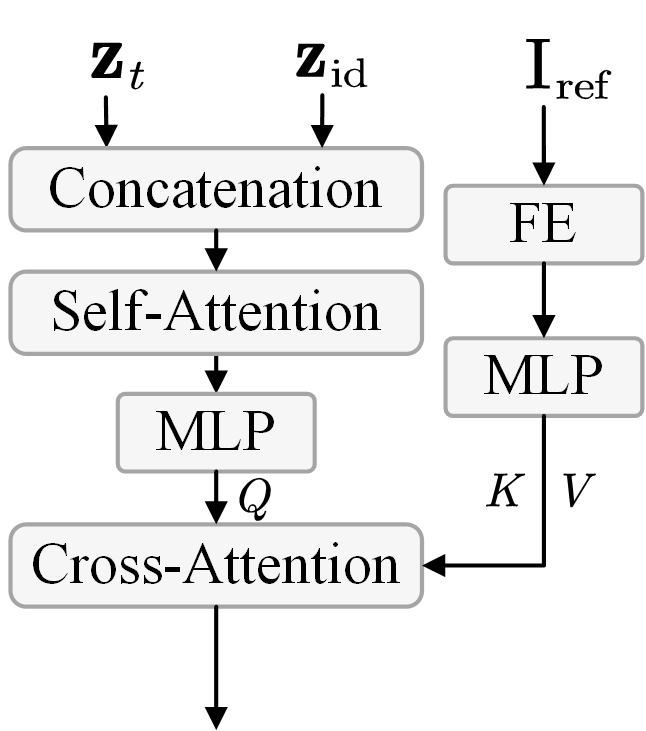
\includegraphics[width=\linewidth]{figs/RefCondition/VAE_CA.png}  
%         \caption{}  
%         \label{fig:RefConditionVAECA}  
%     \end{subfigure}%
%      \label{fig:RefCondition}
%     \caption{{Different strategies of identity conditioning. FE refers to the face encoder. Cross-Attention demonstrates the best performance. (a) Face attention; (b) Face adaptive norm; (c) Identity reference network; (d) Face attention and Identity reference network.}}

% \end{figure}



\noindent\textbf{Identity Reference Network.}  
Diffusion transformer-based video generation models encounter significant challenges in maintaining facial identity coherence, particularly as the length of the generated video increases. 
While incorporating speech audio embeddings as conditional features can establish a correspondence between audio speech and facial movements, prolonged generation often leads to rapid degradation of facial identity characteristics.  

To address this issue, we introduce a control condition within the existing diffusion transformer architecture to ensure long-term consistency of facial identity appearance. 
{We explore four strategies~(as shown in Figure~\ref{fig:IdCondition}) for appearance conditioning: 1) Face attention, where identity features are encoded by the face encoder and combined with a cross-attention module; 2) Face adaptive norm, which integrates features from the face encoder with an adaptive layer normalization technique; 3) Identity reference network, where identity features are captured by a 3D VAE and combined with some transformer layers; and 4) Face attention and Identity reference network, which encodes identity features using both the face encoder and 3D VAE, combining them with self-attention and cross-attention. Our experiments show that the combination with Face attention and Identity reference net achieves the best performance in our model. For further details, please refer to Section~\ref{sec:ablationstudy}. }

We treat a reference image as a single frame and input it into a causal 3D VAE to obtain latent features, which are then processed through a reference network consisting of 42 transformer layers. Mathematically, if \(\mathbf{I}_{\text{ref}}\) denotes the reference image, the encoder function of the 3D VAE is defined as: $\mathbf{z}_\text{id} = \mathcal{E}_{3D}(\mathbf{I}_{\text{ref}})$,
where \(\mathbf{z}_{\text{id}}\) represents the latent features associated with the reference image.  

During the operation of the reference network, we extract vision tokens from the input of the 3D full attention mechanism for each transformer layer, which serve as reference features \(\mathbf{z}_{\text{id}}\). These features are integrated into corresponding layers of the denoising network to enhance its capability, expressed as: $\mathbf{z}_{t, \text{enhanced}} = \text{SelfAttention}(\mathbf{z}_t, \mathbf{z}_{\text{id}}),$
where \(\mathbf{z}_t\) is the latent representation at time step \(t\). 
Given that both the reference network and denoising network leverage the same causal 3D VAE with identical weights and comprise the same number of transformer layers (42 layers in our implementation), the visual features generated from both networks maintain semantic and scale consistency. 
This consistency allows the reference network's features to incorporate the appearance characteristics of facial identity from the reference image while minimizing disruption to the original feature representations of the denoising network, thereby reinforcing the model's capacity to generate coherent and identity-consistent facial animations across longer video sequences.

\noindent\textbf{Temporal Motion Frames.}  
To facilitate long video inference, we introduce the last \(n\) frames of the previously generated video, referred to as motion frames, as additional conditions. Given a generated video length of \(L\) and the corresponding latent representation of \(l\) frames, we denote the motion frames as \(N\). 
The motion frames are processed through the 3D VAE to obtain \(n\) frames of latent codes. 
We apply zero padding to the subsequent \((l-n)\) frames and concatenate them with \(l\) frames of Gaussian noise. 
This concatenated representation is then patchified to yield vision tokens, which are subsequently input into the denoising network. By repeatedly utilizing motion frames, we achieve temporally consistent long video inference.



\subsection{Training and Inference}\label{sec:train}

\noindent\textbf{Training.}  
%The objective of the training process is to minimize the expected mean squared error between actual and predicted noise, framed by the loss function: $\mathcal{L} = \mathbb{E}_{\mathbf{z}_0, \mathbf{c}, \boldsymbol{\epsilon}, t} \left[ \omega(t) \left\| \boldsymbol{\epsilon} - \boldsymbol{\epsilon}_{\theta}(\mathbf{z}_t, t, \mathbf{c}) \right\|_2^2 \right]$, where \(\omega(t)\) serves as a weighting function to balance the loss in various time steps.  
The training process consists of two phases:

\textbf{(1) Identity Consistency Phase.} In this initial phase, we train the model to generate videos with consistent identity. The parameters of the 3D Variational Autoencoder (VAE) and face image encoder remain fixed, while the parameters of the 3D full attention blocks in both the reference and denoising networks, along with the face attention blocks in the denoising network, are updated during training. The model’s input includes a randomly sampled reference image from the training video, a textual prompt, and the face embedding. The textual prompt is generated using MiniCPM\cite{yao2024minicpm}, which describes human appearance, actions, and detailed environmental background. The face embedding is extracted via InsightFace\cite{insightface2024}. With these inputs, the model generates a video comprising 49 frames.

\textbf{(2) Audio-Driven Video Generation Phase.} In the second phase, we extend the training to include audio-driven video generation. We integrate audio attention modules into each transformer block of the denoising network, while fixing the parameters of other components and updating only those of the audio attention modules. Here, the model's input consists of a reference image, an audio embedding, and a textual prompt, resulting in a sequence of 49 video frames driven by audio.
% \text{}(1) In the first phase, we train the model to output videos with consistency of identity. The parameters of the 3D VAE and face image encoder are fixed, while the parameters of the 3D full attention in the reference network, composed of a series of transformer blocks, and those in the denoising network, including the 3D full attention and face attention, are updated through training. The model's input comprises a randomly sampled reference image from the training video, a textual prompt, and the face embedding obtained from the face encoder, with the output being a sequence of 49 frames of video. 
% (2) In the second phase, we train the model for audio-driven video generation. We insert audio attention modules into each transformer block of the denoising network, fixing the parameters of the other components and updating only those of the audio attention modules. The model's input consists of the reference image, input audio, and textual prompt, yielding a sequence of 49 frames of video.

\noindent\textbf{Inference.}  
%After training, new samples can be generated by initializing from a random Gaussian latent vector \(\mathbf{z}_T \sim \mathcal{N}(\mathbf{0}, \mathbf{I})\) and applying the iterative denoising process, defined as: $\mathbf{z}_{t-1} = \frac{1}{\sqrt{\alpha_t}} \left( \mathbf{z}_t - \frac{1 - \alpha_t}{\sqrt{1 - \bar{\alpha}_t}} \, \boldsymbol{\epsilon}_{\theta}(\mathbf{z}_t, t, \mathbf{c}) \right) + \sigma_t \mathbf{n}$, where \(\mathbf{n} \sim \mathcal{N}(\mathbf{0}, \mathbf{I})\) and \(t\) iterates from \(T\) to \(1\). The original image is reconstructed by decoding the final latent vector \(\mathbf{z}_0\) using the VAE decoder, yielding the generated output image represented as \(\mathbf{I} = \mathcal{D}(\mathbf{z}_0)\).  
During inference, the model receives a reference image, a segment of driving audio, a textual prompt, and motion frames as inputs. 
The model then generates a video that exhibits identity consistency and lip synchronization based on the driving audio. 
To produce long videos, we utilize the last two frames of the preceding video as motion frames, thereby achieving temporally consistent video generation.


% \begin{itemize}
%     \item \textbf{Extraction of Single-Speaker Video Clips:}
%     \begin{itemize}
%         \item \textbf{Shot Splitting and Re-encoding}: We employed scene detection and ffmpeg tools to split the videos into individual shots and re-encode them at a frame rate of 25 fps or lower, ensuring synchronization between audio and video data.
%         \item \textbf{Audio Processing}: Utilizing Ultimate Vocal Remover technology, we eliminated background music and environmental sounds from the videos, retaining only the vocal components. This step was crucial for ensuring alignment between audio embeddings and lip movements in the video.
%         \item \textbf{Segment Extraction}: Through the application of pyannote's speaker diarization and overlapped speech detection tools, we accurately extracted segments featuring a single speaker, ensuring that each video clip contained only one speaker's voice.
%     \end{itemize}

%     \item \textbf{Face and Camera Motion Filter:}
%     \begin{itemize}
%     \item **Facial Displacement Filter:** We employed InsightFace technology to calculate facial displacement in the videos, filtering out data where the facial displacement within a 17-frame window exceeded 50\% of the facial bounding box. This step ensured stable character movements and reduced facial blurriness due to rapid motion.
%     \item **Facial Rotation Filter:** Similarly, we utilized InsightFace technology to compute the facial rotation angles, particularly horizontal yaw, filtering out data with an average horizontal rotation exceeding 40°. This measure ensured that the faces in the videos were generally oriented towards the camera.
%     \item ** Camera Motion Filter:** Using CoTracker technology, we detected camera motion classifications in the videos and filtered out data exhibiting dynamic camera movements to minimize interference from moving backgrounds.
%     \item **Audio Lip Sync Filter:** We employed SyncNet technology to compute the audio-visual synchronization scores of the videos, filtering out data with scores below 5.0.
%     \end{itemize}
%     \item \textbf{Data Post-processing:}
%     \begin{itemize}
%         \item **Video Cropping:** Based on the facial positions detected in the previous steps, we cropped the videos into segments with a 3:2 aspect ratio to meet the model's input requirements.
%         \item **Facial Encoding:** A random frame's face was selected, and InsightFace technology was utilized to encode it into embeddings, providing essential facial feature information for the model.
%         \item **Audio Encoding:** The audio from the videos was extracted and encoded into embeddings using Wav2Vec2 technology, facilitating the injection of audio conditions during model training.
%     \end{itemize}
% \end{itemize}

    % \item \textbf{Facial Displacement Calculation:} We employed insightface technology to calculate facial displacement in the videos, filtering out data where the facial displacement within a 17-frame window exceeded 50\% of the facial bounding box. This step ensured stable character movements and reduced facial blurriness due to rapid motion.
    
    % \item \textbf{Facial Rotation Angle Calculation:} Similarly, we utilized insightface technology to compute the facial rotation angles, particularly horizontal yaw, filtering out data with an average horizontal rotation exceeding 40°. This measure ensured that the faces in the videos were generally oriented towards the camera.
    
    % \item \textbf{Camera Motion Classification Detection:} Using CoTracker technology, we detected camera motion classifications in the videos and filtered out data exhibiting dynamic camera movements to minimize interference from moving backgrounds.
    
    % \item \textbf{SyncNet Score Calculation:} We employed SyncNet technology to compute the audio-visual synchronization scores of the videos, filtering out data with scores below 5.0.


\begin{figure*}[t]
    \centering
    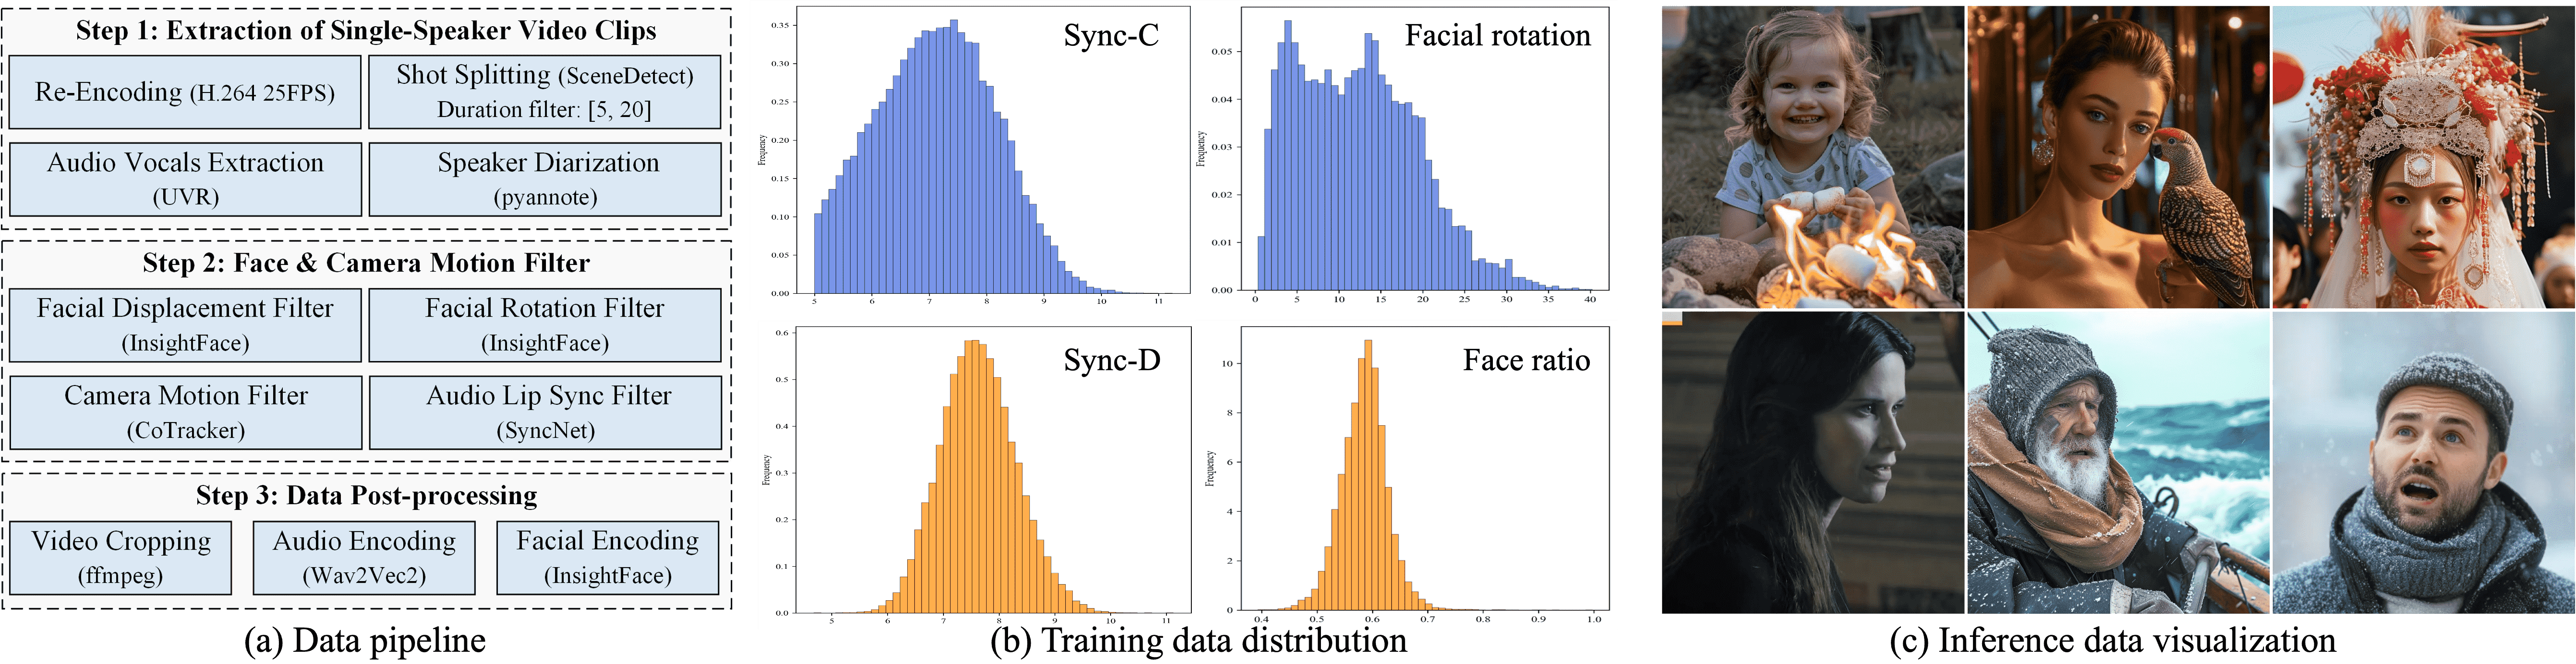
\includegraphics[width=\linewidth]{figs/dataset_comp.png}
    \vspace{-7mm}
    \caption{{
Illustration of the dataset, including the flow of data processing, data distribution across different metric, and the visualization of some representative portrait images for inference.}}
    \label{fig:data_statistics}
    % \vspace{-4mm}
\end{figure*}


\subsection{Dataset}\label{sec:data}



In this section, we will give a detailed introduction of our data curation, including data sources, filtering strategy and data statistics.
Figure~\ref{fig:data_statistics} shows the data pipeline and the statistical analysis of the final data.

\noindent\textbf{Data Sources}
The training data used in this work is prepared from three distinct sources to ensure diversity and generalization. Specifically, the sources are: (1) HDTF dataset~\cite{zhang2021flow}, which contains 8 hours of raw video footage; (2) YouTube data, which consists of 1,200 hours of public raw videos; (3) a large scale movie dataset, which contains film videos of 2,346 hours. 
Our dataset contains a large scale of human identities and, however, we find that YouTube and movie dataset contains  a large amount of noised data. Therefore, we design a data curation pipeline as follows to construct a high-quality and diverse talking dataset, as shown in Figure~\ref{fig:data_statistics}(a).

% \begin{itemize}

%     \item \textbf{HDTF Dataset:} this open-source Talking Face video dataset provides 8 hours of raw video footage. After extensive cleaning and preprocessing, 6 hours of high-quality data are curated for model training.
    
%     \item \textbf{YouTube Data:} We collect 1,200 hours of video data from YouTube, and apply a thorough cleaning process that involved removing duplicates, low-quality videos, and irrelevant content. Finaly, 72 hours of high-quality video are left for training.
    
%     \item \textbf{Film Data:}  To diversify the dataset, we collect and construct a large scale movie video dataset, which contains 2,346 hours. After data curation, 53 hours of video data are retained.
% \end{itemize}



\noindent\textbf{Video Filtering.}
During the data pre-processing phase, we implement a series of meticulous filtering steps to ensure the quality and applicability of the dataset. The workflow includes three stages: extraction of single-speaker, motion filter and post-processing. Firstly, we select video of single-speaker. This stage aims to clean the video content to solve camera shot, background noise, etc, using existing tools~\cite{Plaquet23,Bredin23}. After that, we apply several filtering techniques to ensure the quality of head motion, head pose, camera motion, etc~\cite{karaev23cotracker,karaev24cotracker3,Chung16a}. In this stage, we compute all metric scores for each clip, therefore, we can flexibly adjust data screening strategies to satisfy different data requirement of our multiple training stages or strategies. Finally, based on the facial positions detected in previous steps, we crop the videos to a 3:2 aspect ratio to meet the model's input requirements. We then select a random frame from each video and use InsightFace~\cite{ren2023pbidr} to encode the face into embeddings, providing essential facial feature information for the model. Additionally, we extract the audio from the videos and encode it into embeddings using Wav2Vec2 model~\cite{baevski2020wav2vec}, facilitating the incorporation of audio conditions during model training.

\noindent\textbf{Data Statistics.}
Following the data cleaning and filtering processes, we conducted a detailed analysis of the final dataset to assess its quality and suitability for the intended modeling tasks. Finally, our training data contains about 134 hours of videos, including 6 hours of high-quality data from HDTF dataset, 72 hours of YouTube videos, and 56 hours of movie videos. Figure~\ref{fig:data_statistics}(b) also shows other statistics, such as Lip Sync score~(Sync-C and Sync-D), face rotation, face ratio~(the ratio of face height to video height).
%As can be seen in Fig~\ref{fig:data_statistics}b, our dataset has a large.



